\documentclass[12pt]{article}

\usepackage[english]{babel}
\usepackage[utf8]{inputenc}
\usepackage{amsmath}
\usepackage{graphicx}
\usepackage{setspace}
\usepackage{indentfirst}
\usepackage{apacite}
\usepackage{natbib}
\usepackage{etoolbox}
\usepackage{float}
\usepackage[hyphens,spaces,obeyspaces]{url}
\usepackage{listings}
\usepackage{hyperref}
\usepackage{esvect}
\usepackage[margin=1.25in,letterpaper]{geometry}

% Default fixed font does not support bold face
\DeclareFixedFont{\ttb}{T1}{txtt}{bx}{n}{12} % for bold
\DeclareFixedFont{\ttm}{T1}{txtt}{m}{n}{12}  % for normal

% Custom colors
\usepackage{color}
\definecolor{deepblue}{rgb}{0,0,0.5}
\definecolor{deepred}{rgb}{0.6,0,0}
\definecolor{deepgreen}{rgb}{0,0.5,0}

% Python style for highlighting
\newcommand\pythonstyle{\lstset{
language=Python,
basicstyle=\ttm,
otherkeywords={self},             % Add keywords here
keywordstyle=\ttb\color{deepblue},
emph={MyClass,__init__},          % Custom highlighting
emphstyle=\ttb\color{deepred},    % Custom highlighting style
stringstyle=\color{deepgreen},
frame=tb,                         % Any extra options here
showstringspaces=false            % 
}}

% Python environment
\lstnewenvironment{python}[1][]
{
\pythonstyle
\lstset{#1}
}
{}

% Python for external files
\newcommand\pythonexternal[2][]{{
\pythonstyle
\lstinputlisting[#1]{#2}}}

% Python for inline
\newcommand\pythoninline[1]{{\pythonstyle\lstinline!#1!}}

\title{Assignment Name here}
\author{Author name here}

\begin{document}
\maketitle

\section{First Section}

\subsection{First subsection}
\textbf{Some bold heading} 

Some random matrix

\[
A_{1} = 
\begin{bmatrix}
1 & 1  & 1 &  | & 3   \\ 
1 & 3  & -1 & | & 1  \\ 
3 & 5 & 4 & | & 10
\end{bmatrix}
\]

\begin{center}
Random text in the center
\end{center}

\[ x = 2, y = 0, z = 1\]


\textbf{Some bold text here} 

This is how you write centered equations: \footnote{ \#This\_is\_latex: This is an application of a template in Latex.}

\[x+y+3z=1\]
\[y-7z=1\]

\subsection{Second subsection of first section}

Some text here

\section{Second Section}

\subsection{First subsection}
\textbf{Part (i)-(a):} Some text here along with some equation below:

\[ M_8 M_7 M_6 M_5 M_4 M_3 M_2 M_1 = M_8 M_7 M_6 M_5 M_4 M_3 M_2 M_1 \]

Here is a random matrix on the left of the page:\\

$M_{8} = 
\begin{bmatrix}
1 & 0 & -2 \\ 
0 & 1 & 0 \\ 
0 & 0 & 1
\end{bmatrix}\
$

\section{A new section}

Given the system, we can infer the equations: \citep{Ref1}. I am referring to Figure \ref{fig:colormap}.

\begin{figure}[!h]
\centering
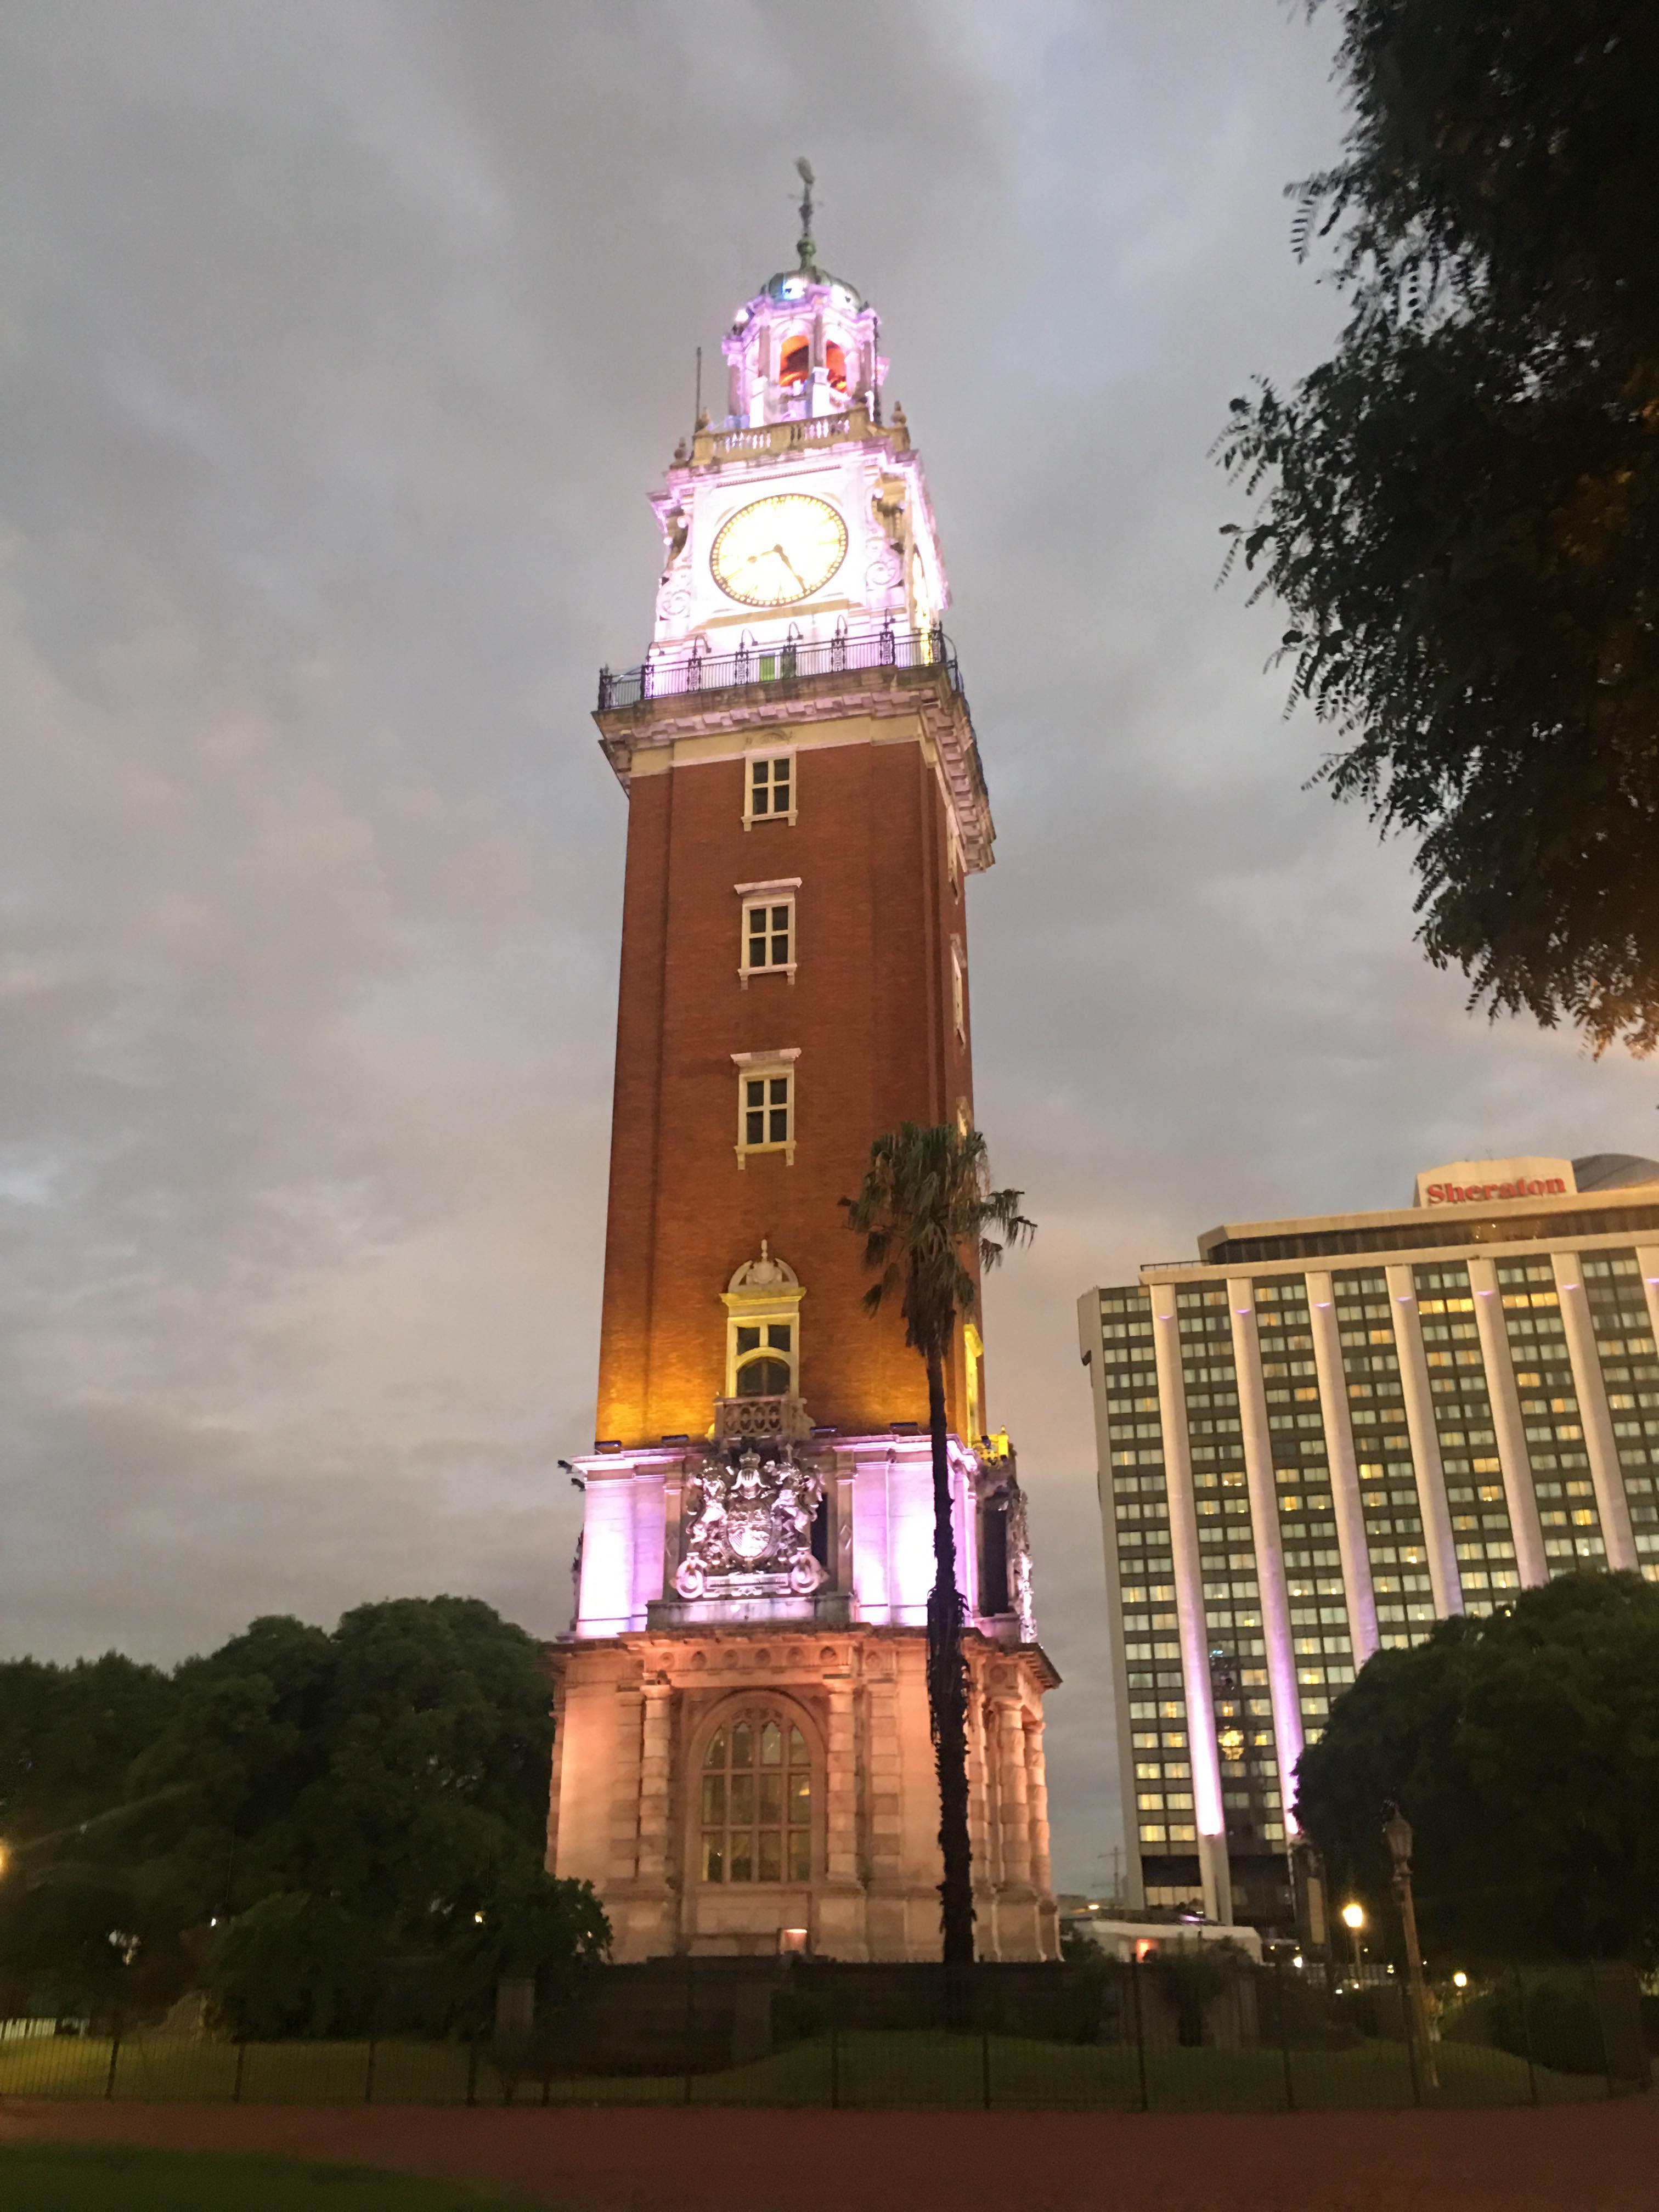
\includegraphics[width=100mm,scale=1]{image.jpg}
\caption{My results from the experiment.}
\label{fig:colormap}
\end{figure}

\section{Appendix}

\subsection{Glossary}

\begin{itemize}
\item First item
\item Second item
\item Third item
\end{itemize}

\subsection{Some Code}
\renewcommand{\baselinestretch}{1}\normalsize
\begin{python}[breaklines,basicstyle=\ttfamily]
import math
x = 2 + 3
v = math.factorial(1)

\end{python}

\subsection{Some more code}
\renewcommand{\baselinestretch}{1}\normalsize
\begin{python}[breaklines,basicstyle=\ttfamily]
import numpy
import pandas
print('Hello World')
\end{python}

\bibliographystyle{apacite}
\bibliography{mybib}

\end{document}